\chapter{序論}
\label{chap:introduction}
\section{背景}

% なぜこの研究が必要だったのか、しっかりした理屈を考えておく。
% 現状どういう問題があるのか
% どういう方法で解決を試みたのか
% 結果として上手く行ったのか、いかなかったのか

近年、スマートフォンなどのモバイルインターネット端末は爆発的に普及し、利用者の年代を問わず用いられるようになった。
もはや生活の一部とも言える存在となったスマートフォンだが、私が日常的に使用する中で不便だと感じる点がある。
それはAndroid Widgetを用いた情報の獲得についてである。
Android Widgetは設置してさえおけばユーザーが能動的に操作をしなくとも、最新の情報を常に画面に表示してくれるので情報の獲得手法としては有効である。

しかし、Android Widgetはいくつかの問題を抱えている。
まずAndroid端末の一つの画面に置くことの出来るAndroid Widgetの数は限られているため、獲得できる情報の種類も限られてしまうという問題である。(図\ref{fig:old_widget})
例えば天気予報を見たければ天気予報のAndroid Widgetを画面に設置し、別の情報が必要であればまた別のAndroid Widgetを設置する必要がある。
Android Widgetの性質上、取得したい情報に付随して不要な情報までもが表示され、それによって画面スペースが埋められてしまうというケースも存在する。
また、自分の取得したい情報に対応したAndroid Widgetが存在しない場合、自らAndroid Widgetを作成する以外の対応策がない。
現状ではAndroid Widgetの作成は多数のスマートフォンユーザーにとって技術的なハードルが高く、問題の解決法としては現実的ではない。

本研究では単体で複数の情報を表示することの出来る汎用的なAndroid Widgetを作成することでこれらの問題の解決を図った。

\begin{figure}[htbp]
  \begin{minipage}{\hsize}
    \begin{center}
      \fbox{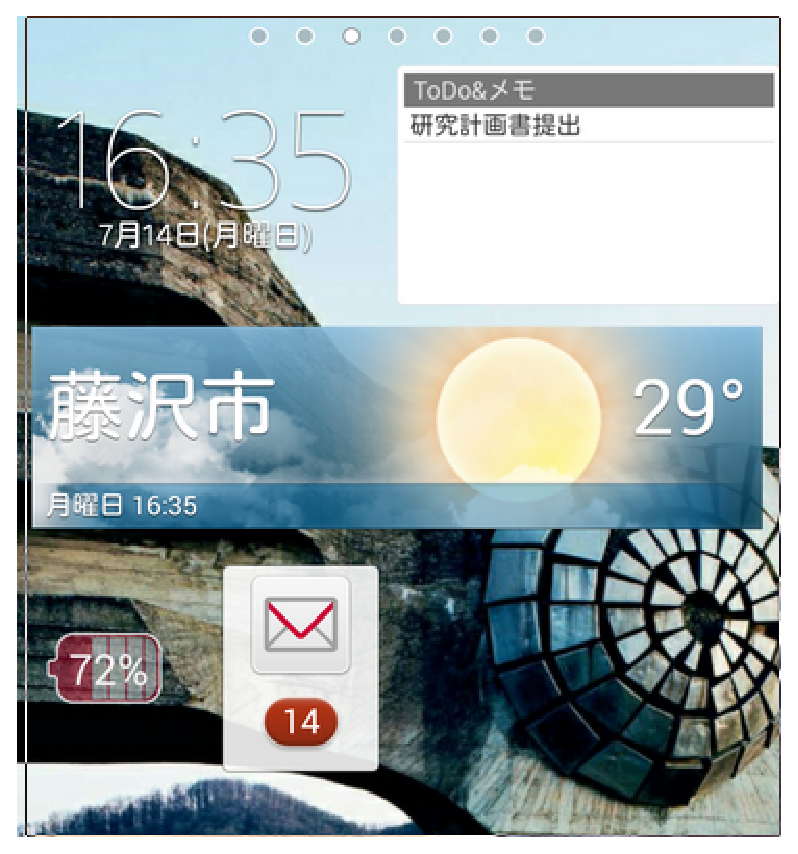
\includegraphics{image/old_widget.eps}}
    \end{center}
    \caption{現状のAndroid Widgetを使用した画面}
    \label{fig:old_widget}
  \end{minipage}
\end{figure}

\section{目的}
%こんな素敵なことが出来るようになるんだよ。
本研究の目的は、ユーザーが必要とする複数の情報を表示するシステム及びインターフェースの実現である。
それによって情報の獲得が容易になり、さらに取得する情報からノイズが減ることになり、ユーザーは効率良く価値の高い情報を得ることが出来るようになる。
%また現状ではAndroid Widgetとして表示することの難しい情報の取得が容易になることで、
%そのため、まずはユーザーが必要とする可能性のある情報を予め取得し、記録しておくことが必要である。次に記録したデータから、ユーザー自らが取得したいデータを選択できるインターフェースを用意し、そこで選択されたデータをユーザーに提供することでユーザーが知りたい情報のみを取得・表示できるインターフェースを実現する。

\section{本論文の構成}
第\ref{chap:introduction}章では本研究の概要を書いた。

第\ref{chap:contents}章では研究内容を説明する。第\ref{chap:prototype}章ではプロトタイプの実装方法を解説する。第\ref{chap:consideration}章では考察を書く。最後に第\ref{chap:conclusion}章にて結論を書き本論文をしめることとする。添付として参考文献を追記する。
